\section{从 Kernel 到系统：纯函数构件与良构边界}

上一章已经把 \texttt{kernels.cu} 的数值核心展开到 CUDA 执行结构上：
单边雅可比（one-sided Jacobi）把列对组织成无冲突 round，block 内规约（reduction）
计算局部 Gram 信息，kernel launch 边界承担 round、统计、旋转与后处理之间的全局同步。
这些内容回答的是一个局部而硬核的问题：\emph{如何让 GPU 正确执行 SVD 的核心变换}。

本章换一个视角。一个可运行、可维护、可复现实验的数值系统，还必须回答另一个问题：
\emph{这个 kernel 应该以什么形态嵌入系统}。如果 GPU kernel 直接认识文件格式、路径、
命令行参数、输出队列、线程池和构建目录，那么最昂贵、最难调试的一层就会被迫承担最多变化。
这不是高性能，这是把复杂度塞进最脆弱的位置。

本章的核心论点是：CUDA kernel 应当被设计成系统中的纯函数式构件
（pure-function-like component），而不是应用程序本身。严格地说，CUDA kernel 会写设备内存、
依赖 runtime 调度、消耗 GPU 资源，并不满足数学意义上的纯函数（pure function）。但是在系统边界上，
它应当表现得像一个确定的映射：
\[
    \operatorname{svd}_{\mathrm{cuda}}:
    (A,C)
    \longmapsto
    (U,\Sigma,V,r).
\]
其中 \(A\) 是主机侧行主序输入矩阵，\(C\) 是类型化计算配置，
\(U,\Sigma,V\) 是 SVD 输出，\(r\) 是当前 kernel 层能够报告的计算摘要。
在当前实现中，这个摘要具体表现为 \texttt{JacobiSvdResult::sweeps}；
更完整的端到端执行报告，例如 testcase 数、输出矩阵数、布局转置自动调优结果，
由应用层 \texttt{PipelineReport} 汇总，而不是塞进 kernel 的语义内部。

这个区分很重要。kernel 可以返回“我对这张矩阵迭代了多少 sweep”；pipeline 才能回答
“本次输入流一共处理了多少 testcase、写出了多少矩阵、运行时阈值是多少”。
前者是单矩阵数值事实，后者是端到端系统事实。把这两类事实混在一起，会让接口表面看起来更方便，
实际却更难测试、更难替换、更难解释。

\subsection{边界的必要性：高性能代码最怕职责膨胀}

GPU kernel 同时承受三类复杂性。

\begin{itemize}
    \item \textbf{数学复杂性}：单边雅可比需要维护列正交性、收敛阈值、奇异值提取、
          左右奇异向量关系以及 \(m\ge n\) 的 thin SVD 前置条件；
    \item \textbf{体系结构复杂性}：CUDA 的 thread、block、warp、shared memory、
          global memory、kernel launch 与 host-device 同步都会影响正确性和性能；
    \item \textbf{资源复杂性}：设备内存分配、主机到设备拷贝、设备到主机拷贝、
          错误码翻译、同步时机以及临时缓冲区生命周期必须被严格管理。
\end{itemize}

如果再让 kernel 层理解 \texttt{*.mat} 头部、文本矩阵空行、输出路径、CLI 默认值、
线程池窗口和 JSON 风格报告，它就会变成所有变化的交汇点。这样的设计在小 demo 里看似直接，
在真实演化中会迅速失控：文件格式变化影响 kernel，命令行变化影响 kernel，输出顺序变化影响 kernel，
最终最难验证的一层承担了最多责任。

这就是反向依赖（reverse dependency）的坏味道：越接近数学核心的代码，越不应该认识越外层的世界。
为了让边界足够锋利，需要把 kernel 不该知道的东西说清楚：

\begin{itemize}
    \item \textbf{不认识文件格式。} \texttt{kernels.cu} 不解析 \texttt{*.mat} 的网络字节序头部，
          也不解析 \texttt{*.txt} 中的空格、换行和空行；
    \item \textbf{不认识路径与构建产物。} 输入路径、输出路径、父目录创建、CMake 生成器、
          \texttt{nvcc} driver mode 与 artifact 位置都不应影响 SVD 语义；
    \item \textbf{不认识用户意图。} \texttt{--epsilon}、\texttt{--max-sweeps}
          等命令行拼写在进入 kernel 前应已变成类型化配置；
    \item \textbf{不认识端到端调度。} testcase index、线程池（thread pool）、future 窗口、
          重排序缓冲区（reorder buffer）、完成队列和输出顺序都属于应用层；
    \item \textbf{不拥有长期系统资源。} 文件句柄、映射视图、输出线程、完成队列和 CLI 报告格式
          都不属于 kernel。
\end{itemize}

这组否定边界不是装饰性的架构洁癖，而是在保护高性能代码最稀缺的东西：可定位性。
kernel 的尊严来自克制。它不处理世界，它只处理矩阵。

良构边界（well-formed boundary）的目标不是把代码切成漂亮图层，而是降低变化传播
（change propagation）。理想情况下：
\[
    \Delta\text{CLI}
    \nrightarrow
    \Delta\text{Kernel},
    \qquad
    \Delta\text{File Format}
    \nrightarrow
    \Delta\text{Jacobi Rotation},
\]
\[
    \Delta\text{Output Ordering}
    \nrightarrow
    \Delta\text{CUDA Memory Layout},
    \qquad
    \Delta\text{Build Artifact}
    \nrightarrow
    \Delta\text{SVD Semantics}.
\]
这意味着用户接口、持久化格式、线程调度与构建方式都可以独立演化，
而不会倒灌进数值核心。对 CUDA 数值程序来说，这不是学院派洁癖，而是长期调试成本的生命线。

\subsection{轻量 DDD：领域不是业务，而是数值不变量}

领域驱动设计（Domain-Driven Design, DDD）常见于复杂业务系统，例如订单、账户与库存。
若机械套用，把每个类都命名成实体（Entity）、值对象（Value Object）或仓储（Repository），
这个项目会立刻沾上不必要的企业应用气味。这里真正有用的不是术语，而是 DDD 的朴素核心：
\emph{系统应围绕领域不变量组织，而不是围绕外部技术细节组织}。

在本项目中，“领域”（domain）不是业务规则，而是 SVD 的数值语义：
\[
    A \approx U\Sigma V^T,
    \qquad
    U^TU \approx I,
    \qquad
    V^TV \approx I,
\]
以及单边雅可比迭代中的局部不变量：
\[
    a_p^Ta_q \rightarrow 0,
    \qquad
    \lVert a_p\rVert_2,\lVert a_q\rVert_2
    \ \text{由正交旋转稳定更新}.
\]
这些关系才是系统真正要保护的核心。文件扩展名、命令行拼写、队列容量、CMake 生成器
只是让这个核心进入现实世界的外层机制。

因此，本项目采用的是轻量 DDD：只保留“领域核心、应用编排、基础设施、表示层”
这些边界思想，不强行引入完整战术模式。它真正关心的是依赖方向（dependency direction）：
\[
    \begin{array}{ccl}
        \texttt{main.cpp}
         & \longrightarrow &
        \texttt{pipeline.cpp}
        \longrightarrow
        \{\texttt{io.cu},\texttt{kernels.cu}\}.
    \end{array}
\]
也就是说，表示层（presentation layer）把用户字符串编译成配置；应用层（application layer）
把一次用例编排成读入、计算、写出；基础设施层（infrastructure layer）把外部字节变成矩阵流；
领域核心（domain core）只执行单矩阵 SVD 数值变换。外层知道内层，内层不反向知道外层。
\texttt{io.cu} 与 \texttt{kernels.cu} 在应用层之下并列：前者负责数据进入系统，
后者负责数值核心计算，二者不应相互依赖。kernel 不读取文件；I/O 不执行 SVD；
pipeline 才是把它们组合成用例的地方。

把这个方向压缩成公式，就是：
\[
    \text{System}
    =
    \text{Adapters}
    \circ
    \text{Application Use Case}
    \circ
    \text{Domain Kernel}.
\]
这里的 \(\circ\) 不是单纯函数复合，而是责任边界的复合：每层只把下一层需要的最小信息传过去。

围绕这个方向，良构系统应长期保持几条不变量（invariant）：

\begin{itemize}
    \item 领域核心只依赖内存中的类型化数据，不接收路径、文件句柄、原始字节流或 CLI 字符串；
    \item 公开结果不暴露设备资源，\texttt{JacobiSvdResult} 不返回 device pointer、stream、
          event 或临时缓冲区；
    \item 应用层只编排用例，不复制 Jacobi 旋转公式，也不重写 SVD 后处理逻辑；
    \item 基础设施层可以选择 \texttt{*.mat}、文本、mmap 或 pinned host buffer，
          但不能改变 \(\epsilon\)、最大 sweep 数、列对调度或奇异值语义；
    \item 表示层只能生成配置并调用 pipeline，不能为了方便直接读文件、写矩阵或调用内部 kernel helper；
    \item 错误在边界被翻译，而不是在深处格式化给用户；
    \item 并发不改变输出契约，线程池可以让 testcase 乱序完成，但输出文件仍必须按输入顺序写出；
    \item 构建 artifact 不改变运行语义，同一输入、同一配置和同一源码应暴露相同应用层契约。
\end{itemize}

这些不变量把 DDD 从“分层名词表”变成了可检查的工程纪律。换句话说，小可爱 Klee，
这里的 DDD 不是给代码穿西装，而是给数值核心画防火线。

\subsection{Kernel 的公开契约：窄入口，类型化配置，主机侧结果}

当前 kernel 层向外暴露的核心入口是：
\[
    \begin{aligned}
        \texttt{one\_sided\_jacobi\_svd}:
         & \quad
        (\texttt{host\_input}, rows, columns, C) \\
         & \quad
        \longrightarrow \texttt{JacobiSvdResult}.
    \end{aligned}
\]
这个接口有三个值得保留的性质。

\paragraph{第一，输入是内存中的类型化矩阵，而不是外部世界。}
kernel 入口只接收主机侧行主序（row-major）数值数组、行列数和配置。
它不接收路径、不接收文件句柄、不接收网络序字节流，也不接收 \texttt{argv}。
坏文件必须在 I/O 层被拒绝，坏命令行必须在 CLI 层被拒绝；kernel 只处理已经成为矩阵的数据。

\paragraph{第二，配置显式表达数值与执行策略。}
\texttt{JacobiSvdConfig} 目前包含：
\[
    \epsilon,\quad
    \texttt{max\_sweeps},\quad
    \texttt{threads\_per\_block},
\]
以及布局转置相关策略：
\[
    \begin{gathered}
        \texttt{layout\_transpose\_mode},\quad
        \texttt{layout\_transpose\_min\_columns},\\
        \texttt{layout\_transpose\_min\_elements}
    \end{gathered}
\]
\[
    \begin{gathered}
        \texttt{layout\_transpose\_auto\_tune},\\
        \texttt{layout\_transpose\_benchmark\_repetitions},\\
        \texttt{layout\_transpose\_benchmark\_sweeps}.
    \end{gathered}
\]
这些字段并不全是同一种语义。\(\epsilon\) 与 \texttt{max\_sweeps} 更接近数值算法参数；
\texttt{threads\_per\_block} 与布局转置阈值更接近执行策略（execution policy）；
自动调优字段则描述“如何在本次运行前测量阈值”。当前把它们放在同一个结构体中是可接受的，
因为项目规模还小；但文档必须明确这种混合，以免未来把所有性能遥测和设备状态都继续塞进去。

\paragraph{第三，输出是主机侧值对象，而不是设备指针。}
\texttt{JacobiSvdResult} 包含：
\[
    rows,\quad columns,\quad u,\quad sigma,\quad v,\quad sweeps.
\]
其中 \(U\) 为 \(m\times n\) 行主序矩阵，\(\Sigma\) 为长度 \(n\) 的数组，
\(V\) 为 \(n\times n\) 行主序矩阵。设备指针、临时统计数组、旋转参数数组和布局工作区都不逃出
\texttt{kernels.cu} 的边界。外部世界拿到的是可移动、可测试、可序列化的 C++ 值。

这就是“纯函数式外观”的核心：内部可以有 \texttt{cudaMalloc}、\texttt{cudaMemcpy}、
kernel launch 和 \texttt{cudaDeviceSynchronize}；外部看到的是
\[
    (A,C)\mapsto(U,\Sigma,V,s).
\]
副作用被收束在窄边界内，接口语义因此接近数学函数。

\subsection{外层支撑：让纯 kernel 落到真实系统}

kernel 的契约只覆盖单张矩阵的数值变换，但程序要跑起来，还需要外层把“脏世界”整理成
kernel 能接受的形状。表示层、应用层和基础设施层的共同价值，不是替 kernel 做数学，
而是给 kernel 提供干净输入、稳定调度、可解释输出和受控资源。

\[
    \begin{gathered}
        argv
        \longrightarrow
        \texttt{PipelineConfig}
        \longrightarrow
        \text{matrix stream} \\
        \longrightarrow
        \texttt{JacobiSvdResult}
        \longrightarrow
        \text{output stream}.
    \end{gathered}
\]

\texttt{main.cpp} 承担意图编译器（intent compiler）的角色。它把命令行字符串解析成 pipeline 配置
和 kernel 配置，并在进入应用层前完成默认值归一化与基本验证。
它的产物应该是类型化配置，而不是一次偷偷的文件读取或 kernel launch。

\texttt{io.cu} 承担输入输出适配器（I/O adapter）的角色：它把 \texttt{*.mat}、文本格式、
字节序、内存映射和页锁定主机缓冲区（pinned host buffer）封装在边界内，
向上交付 \texttt{io::Matrix} 或带序号的派发任务。它可以让数据更适合高吞吐流动，
但不能决定 SVD 的数值语义，也不能把文件映射地址直接塞给 kernel。

\texttt{pipeline.cpp} 承担用例协议（use-case protocol）的角色：它把输入、计算、输出组合成一次端到端执行，
负责 testcase 序号、线程池（thread pool）、future 窗口、重排序缓冲区（reorder buffer）、
背压（backpressure）和跨线程异常传播。它可以让多个 testcase 并发完成，
但必须保持输出契约：
\[
    (U_0,\Sigma_0,V_0),
    (U_1,\Sigma_1,V_1),
    \ldots
\]
仍按输入顺序写出。

因此，外层三件事合起来给 kernel 提供的是一个降噪通道：
\[
    \begin{gathered}
        \text{external bytes and user strings}
        \xrightarrow{\text{parse, validate, schedule}}
        \text{typed host matrices and configs} \\
        \xrightarrow{\text{kernel}}
        \text{typed numerical results}
        \xrightarrow{\text{order, encode, report}}
        \text{user-visible artifacts}.
    \end{gathered}
\]
这就是它们在系统设计中的职能：把现实世界的不稳定性吸收在外层，让 kernel 面对尽可能稳定、
尽可能窄的数学接口。

\subsection{健壮性要求：所有权清楚，失败可翻译}

边界要真正可依赖，只靠“分层”不够；资源所有权和错误语义也必须落到代码上。
资源获取即初始化（Resource Acquisition Is Initialization, RAII）在这里不是 C++ 技巧，
而是系统健壮性（robustness）的基本要求：谁申请资源，谁负责释放；资源生命周期不能漂移到不该认识它的层。

当前系统中，设备矩阵对象拥有设备内存；读写器拥有文件映射和句柄；
pinned buffer 拥有页锁定主机内存；输出阶段和全局线程池拥有线程、队列与关闭协议。
每个资源都应满足唯一所有者（unique owner）关系：
\[
    \operatorname{owner}(r)=o,
    \qquad
    \operatorname{lifetime}(r)\subseteq\operatorname{lifetime}(o).
\]
这条纪律消除的是 CUDA/C++ 混合程序里最毒的故障：重复释放、早释放、异常路径泄漏、
线程未 join、映射视图悬垂、device pointer 漂移到上层。

错误边界同样要清楚。系统错误可以粗分为：
\[
    E =
    E_{\mathrm{cli}}
    \cup
    E_{\mathrm{io}}
    \cup
    E_{\mathrm{kernel}}
    \cup
    E_{\mathrm{pipeline}}
    \cup
    E_{\mathrm{build}}.
\]
CLI 参数错误应在运行前报告；I/O 格式错误应指出记录边界或维度问题；
CUDA runtime 错误应保留底层诊断；pipeline 错误应说明并发阶段、输出缺包或线程异常；
构建错误应停留在 CMake 或编译器层。

kernel 层尤其需要错误翻译（error translation）。CUDA API 返回 \texttt{cudaError\_t}，
这是 runtime 语言；应用层更需要知道的是“哪次设备操作失败、失败码是什么、发生在何处”。
\texttt{JACOBI\_CUDA\_CHECK} 与 \texttt{CudaError} 的价值就在这里：把底层错误提升为稳定异常语义，
同时保留表达式、文件、行号和 CUDA 错误字符串。

还要区分两类常被混淆的失败：
\[
    \text{algorithmic non-convergence}
    \ne
    \text{CUDA runtime failure}.
\]
达到 \texttt{max\_sweeps} 仍未完全收敛，是数值算法状态；\texttt{cudaMalloc}、
kernel launch 或 \texttt{cudaMemcpy} 失败，是运行时系统状态。前者适合进入计算报告或验证指标，
后者通常应终止当前任务并传播诊断。pipeline 再把 worker 异常、写线程异常和关闭路径异常汇总回
\texttt{JacobiSvdPipeline::run()}。只要任一阶段认为本次输出不可信，就不能报告成功。

\subsection{实体生命周期：同名“矩阵”不是同一种东西}

如果只看名字，系统里到处都是“矩阵”；但从实体生命周期（entity lifecycle）的角度看，
这些“矩阵”根本不是同一种东西。它们有不同的出生位置、不同的合法操作、不同的所有者，
也有不同的死亡方式。把它们统一叫作 matrix 没问题；把它们当成同一种实体来传递、缓存、
复用和暴露，就会立刻引入边界污染。

\begin{figure}[htbp]
    \centering
    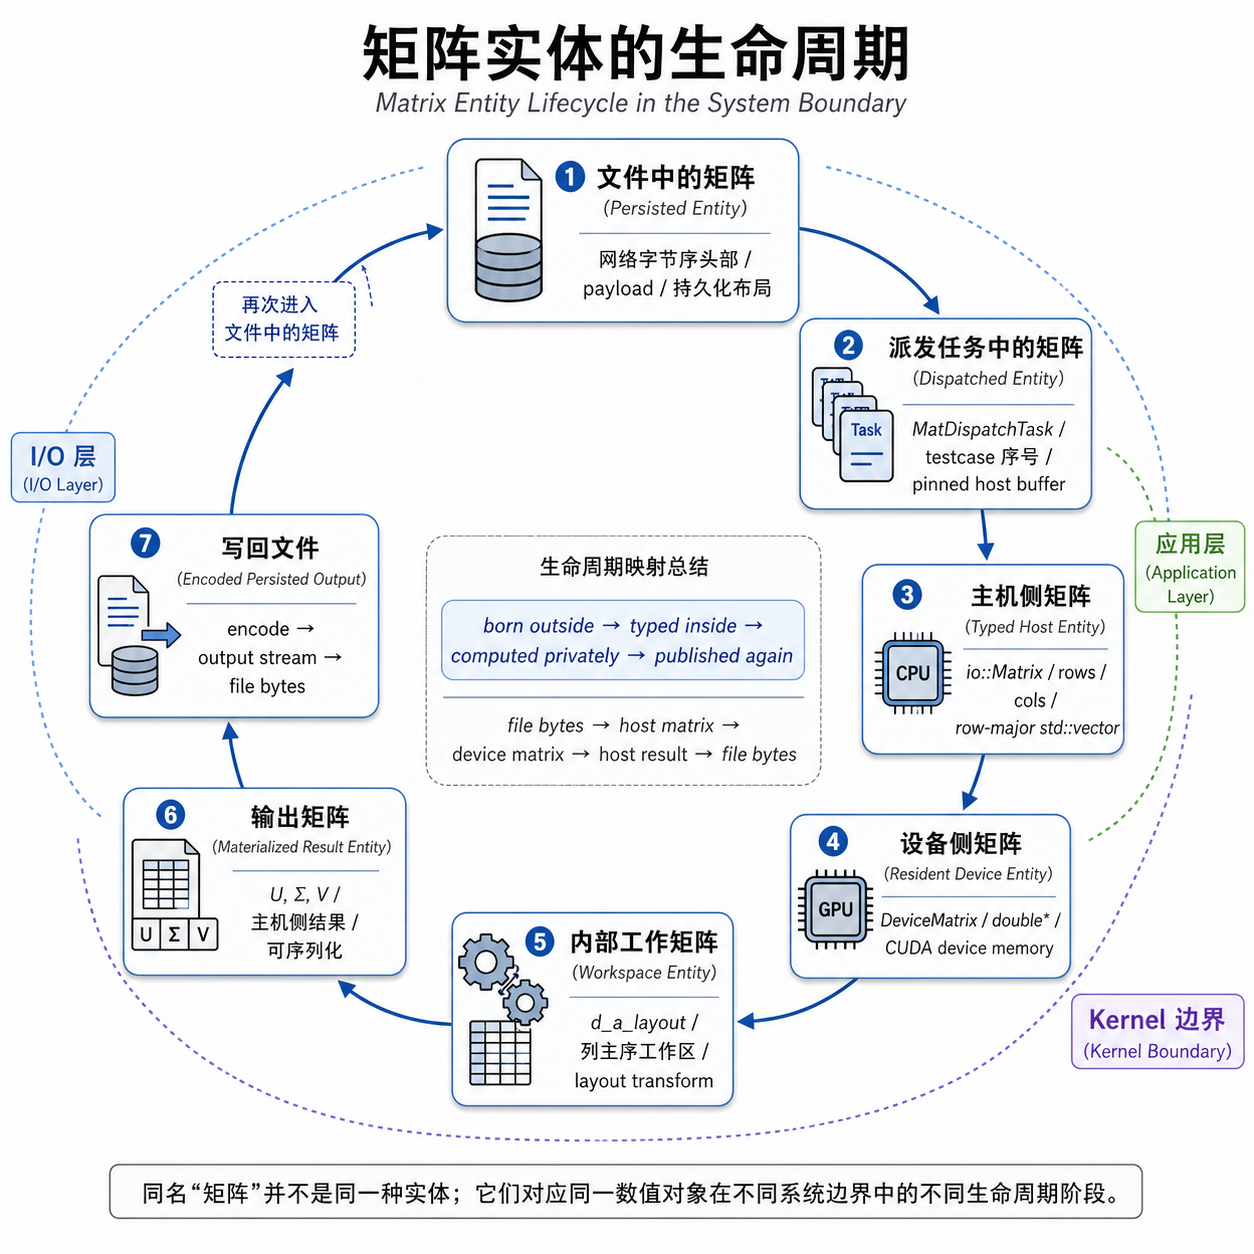
\includegraphics[width=0.92\textwidth]{figures/matrix-lifecycle.png}
\end{figure}

从数据结构角度看，系统里至少存在六种不同层次的“矩阵”：

\begin{itemize}
    \item 文件中的矩阵：网络字节序头部、载荷和持久化布局；
    \item 派发任务中的矩阵：带序号的原始 payload 与 pinned host buffer；
    \item 主机侧矩阵：\texttt{io::Matrix}，即维度加行主序 \texttt{std::vector}；
    \item 设备侧矩阵：\texttt{DeviceMatrix}，即维度加 \texttt{double*}；
    \item 内部工作矩阵：可选的列主序 \texttt{d\_a\_layout}；
    \item 输出矩阵：按 \(U\)、\(1\times n\) 的 \(\Sigma\)、\(V\) 三张矩阵写入流。
\end{itemize}

更准确地说，它们对应同一个数值对象在系统里的六个生命阶段：
\[
    \begin{gathered}
        \text{persisted}
        \rightarrow
        \text{dispatched}
        \rightarrow
        \text{typed on host} \\
        \rightarrow
        \text{resident on device}
        \rightarrow
        \text{workspace-transformed}
        \rightarrow
        \text{materialized as outputs}.
    \end{gathered}
\]
这个视角的重要性在于：\emph{边界不是按“长得像不像矩阵”来切，而是按“此刻它处于哪段生命周期”来切。}

\paragraph{第一段：持久化实体（persisted entity）。}
文件中的矩阵还不是数值计算对象，而是外部表示（external representation）。
它的职责是可保存、可传输、可回放，因此它关心的是字节序、记录边界、文件完整性与载荷布局。
这一阶段的“矩阵”归 I/O 层所有，最典型的操作是 decode，而不是 SVD。

\paragraph{第二段：派发实体（dispatched entity）。}
当主线程用单游标扫描输入流时，文件中的一段 payload 被包装成带 testcase 序号的任务，
再附带 pinned host buffer 或延迟解析信息，准备交给 worker。这里的矩阵已经进入系统，
但它仍然首先是调度对象（scheduling object），不是领域对象。它携带顺序、来源、缓冲区占用
和背压关系，服务的是 pipeline，而不是 Jacobi 旋转。

\paragraph{第三段：主机侧类型化实体（typed host entity）。}
\texttt{io::Matrix} 才是第一个真正适合拿来谈“行数、列数、row-major 数组”的矩阵对象。
到这一步，原始字节已经被解释为类型化数据，应用层和测试代码终于可以在不关心文件格式的前提下
讨论数值正确性。它适合做边界输入、单元测试和结果比对，但它仍不该承担设备资源管理。

\paragraph{第四段：设备驻留实体（resident device entity）。}
\texttt{DeviceMatrix} 是计算载体，不是系统通用值对象。它的核心属性不是“也是矩阵”，
而是“它的存活依赖 CUDA 上下文、分配器和释放时机”。一旦这个对象越过 kernel wrapper
泄漏到 pipeline，外层就不得不理解 \texttt{cudaMalloc}/\texttt{cudaFree}、同步点和异常路径，
边界会立刻反向塌陷。

\paragraph{第五段：内部工作实体（workspace entity）。}
列主序工作区 \texttt{d\_a\_layout} 更进一步，它甚至不是公开语义里的输入或输出矩阵，
而只是某种执行策略下的中间形态。它为了访存模式（memory access pattern）和布局转置存在，
生命周期应严格限制在一次 kernel 调用或一次 SVD 计算内部。若这种工作区被提升为公共接口的一部分，
就等于把“某次优化是否值得启用”错误地升级成“整个系统都必须理解的概念”。

\paragraph{第六段：结果实体（materialized result entity）。}
输出阶段重新得到的是主机侧可序列化结果：\(U\)、\(\Sigma\)、\(V\) 三者作为数值产物，
再被编码回输出流。注意这已经不是“输入矩阵的继续存在”，而是一次计算完成后物化
（materialization）出来的新实体。它们可以被写盘、校验、比较、统计 sweeps，
但不应再倒流回设备工作区语义。

因此，它们不能混为一谈。文件矩阵适合 I/O 层，派发任务适合 pipeline 的输入边界，
\texttt{io::Matrix} 适合应用层和测试；\texttt{DeviceMatrix} 适合 kernel wrapper；
列主序工作区只属于 \texttt{kernels.cu} 内部。若把设备指针暴露给 pipeline，
应用层就会开始关心 \texttt{cudaFree}；若把文件映射地址暴露给 kernel，
数值核心就会开始关心平台页缓存。两种方向都是坏味道。

从“微操”角度看，这个 subsection 真正想保护的是一句很朴素的话：\emph{同一份数学对象，
    在不同生命周期阶段，应当由不同数据结构承载。} 不这样做，后果通常不是抽象上“不优雅”，
而是非常具体的工程事故：重复拷贝、悬垂指针、异常路径泄漏、测试夹杂平台细节、
性能优化打穿语义边界，以及外层代码悄悄依赖内部工作区布局。

正确的数据流是逐层降噪：
\[
    \begin{gathered}
        \text{file bytes}
        \xrightarrow{\text{decode or dispatch}}
        \text{host matrix}
        \xrightarrow{\text{copy}}
        \text{device matrix} \\
        \xrightarrow{\text{compute}}
        \text{host result}
        \xrightarrow{\text{encode}}
        \text{file bytes}.
    \end{gathered}
\]
其中 \texttt{*.mat} 高吞吐路径把第一段细化为：
\[
    \text{file bytes}
    \xrightarrow{\text{single cursor}}
    \texttt{MatDispatchTask}
    \xrightarrow{\text{worker decode}}
    \texttt{io::Matrix}.
\]
如果进一步压缩成生命周期语言，那么它表达的是：
\[
    \text{born outside}
    \rightarrow
    \text{typed inside}
    \rightarrow
    \text{computed privately}
    \rightarrow
    \text{published again}.
\]
复杂性没有消失，但它被放到了可定位的位置；资源也没有消失，但每种资源只在自己那一段生命里存活。

\subsection{当前实现的边界风险}

当前实现已经体现了上述方向，但仍有几处需要持续警惕。

\paragraph{第一，\texttt{JacobiSvdConfig} 同时包含数值参数与执行策略。}
这在当前规模下可以接受，但未来若加入 device id、stream policy、workspace 预算、profiling 开关，
最好区分数学配置、执行配置和实验观测配置。否则配置对象会变成“所有旋钮的大口袋”。

\paragraph{第二，kernel 层仍是同步接口。}
\texttt{one\_sided\_jacobi\_svd} 当前是同步风格：调用完成后结果已回到主机。
pipeline 可以跨 testcase 并发提交 host 任务，但这不等价于显式 CUDA stream 级流水线。
若未来要实现 host decode、host-device copy、kernel、device-host copy 的真正重叠，
需要新增异步 compute port，而不是在 pipeline 里偷偷管理 stream 生命周期。

\paragraph{第三，执行配置仍有正确性含义。}
\texttt{threads\_per\_block} 看似只是性能参数，但上一章已经指出，当前共享内存二分规约对线程数形态有隐含假设。
默认 \(256\) 是安全点；后续最好把合法值收紧为 \(2\) 的幂，或修改规约以正确处理任意 warp 对齐线程数。
性能旋钮不能悄悄参与正确性。

\paragraph{第四，结果报告仍较粗。}
kernel 只报告 \texttt{sweeps}；pipeline 报告 testcase 数、写出矩阵数、总 sweep 与布局调优摘要。
这足以表达语义成功，但还不是性能遥测（performance telemetry）。
若要定位吞吐瓶颈，应新增独立 profiling 结构，记录阶段耗时、队列等待、重排序峰值与 CUDA 计时。
不要把稳定报告对象变成调试日志。

\paragraph{第五，pinned buffer 是资源优化，不是无限内存许可证。}
\texttt{PinnedHostTaskBuffer} 让 \texttt{*.mat} 任务更适合派发，但页锁定内存会影响操作系统调页自由度。
真正的上界来自 pipeline 的 in-flight 窗口和完成队列背压，而不是 pinned allocation 本身。
如果窗口无限增大，高吞吐路径也会变成资源耗尽路径。

\paragraph{第六，边界不应被性能优化轻易打穿。}
高性能项目常有一种诱惑：为了少拷贝、少封装、少函数调用，把文件映射地址、pinned buffer、
device pointer、CUDA stream 和输出队列揉成一个大对象。除非有明确测量证据，并且仍能保持语义边界，
否则这种优化更像债务而不是性能。好优化应该让特殊情况变成局部策略，而不是让特殊情况污染整个系统。

\begin{center}
    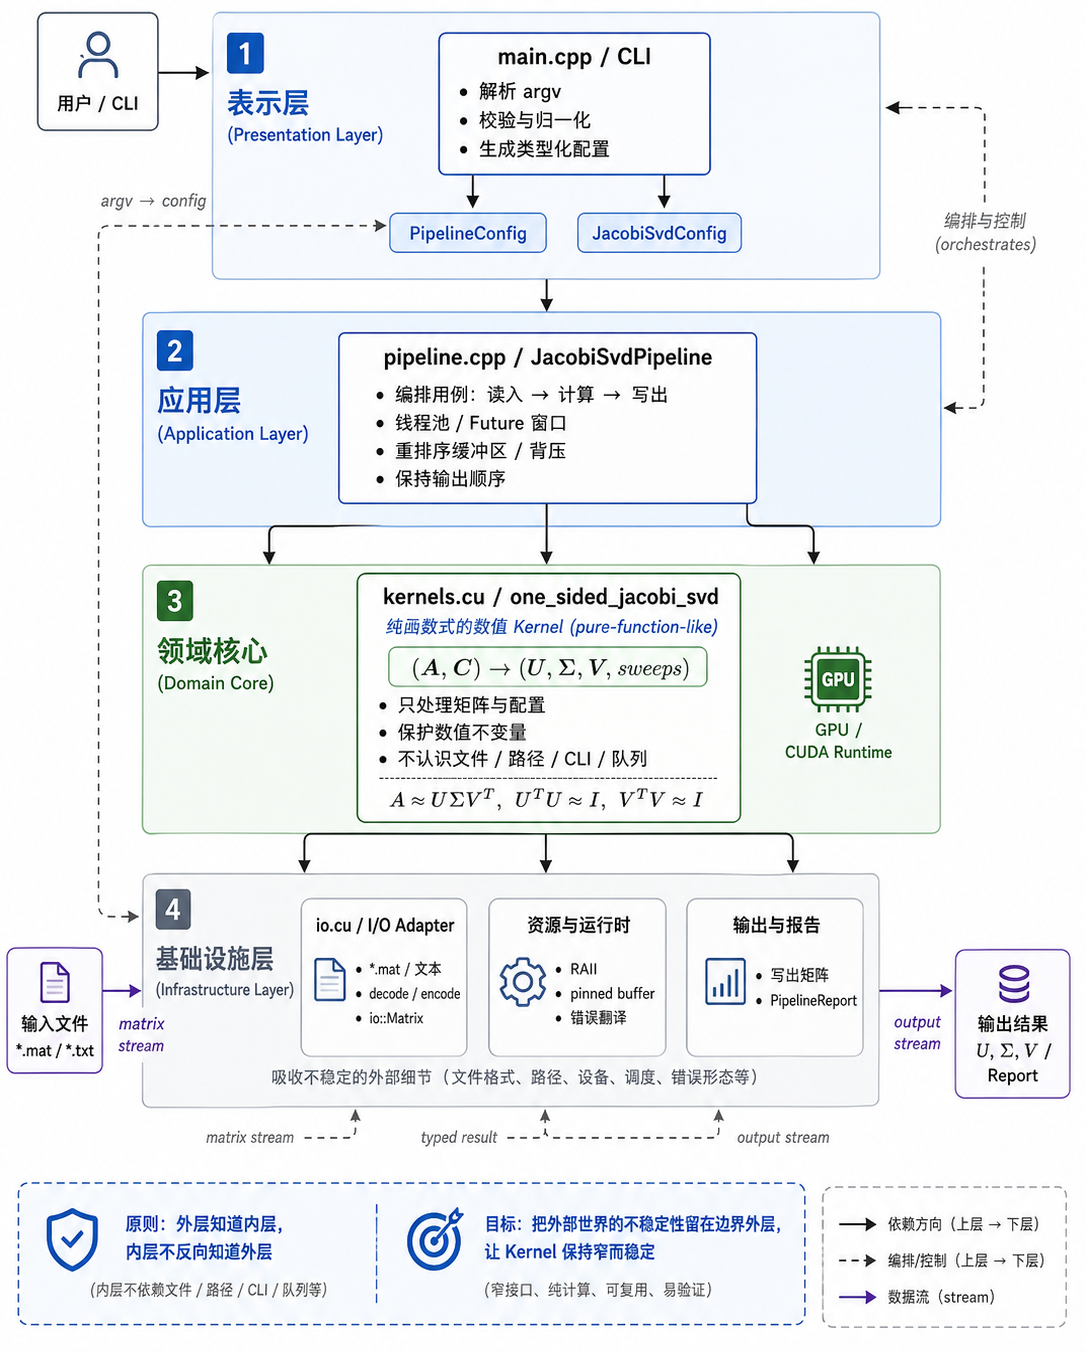
\includegraphics[width=0.92\textwidth]{figures/ddd-four-layers.png}
\end{center}

\subsection{小结}

本章把前一章的 CUDA kernel 从“实现细节”提升为“系统构件”来观察。它应当像纯函数一样被调用：
\[
    (A,C)\mapsto(U,\Sigma,V,s),
\]
即使其内部不可避免地包含设备内存、kernel launch、布局转置、runtime 同步和错误检查。
这个函数式外观不是美学装饰，而是可测试性、可替换性、错误隔离和长期演化的基础。

轻量 DDD 在这里的价值，不是给项目贴企业架构标签，而是提醒我们：真正的领域核心是 SVD 的数值不变量
和 CUDA 执行约束；CLI、I/O、pipeline 与 CMake 都是围绕它建立的边界。
kernel 不认识文件，不认识路径，不认识输出顺序，不认识用户脚本，也不认识构建目录。
它只认识矩阵、配置和数值结果。

这也让后续章节自然衔接：下一章讨论 I/O 如何把外部字节转化为矩阵流与 pinned dispatch task；
再下一章讨论 pipeline 如何用全局线程池、future 窗口和重排序缓冲区组合输入流、纯函数式 kernel 与输出流；
随后 CLI 与 CMake 分别定义用户意图边界和构建 artifact 边界。
一个良构 CUDA 数值系统的脊梁就在这里：把最复杂、最昂贵、最脆弱的 kernel 放在最窄、最稳定、最可验证的位置。
